\documentclass{article}
%
\usepackage[utf8]{vietnam}
\usepackage[a4paper, top=2cm, left=2cm, right=2cm, bottom=2cm]{geometry}
\usepackage{amsmath}
\usepackage{setspace}
\usepackage{graphicx}
\usepackage{icomma}
\usepackage{scrextend}
\usepackage{siunitx}
\usepackage{fancyhdr}
\usepackage{subfigure}
\usepackage{multirow}
%
\changefontsizes{13pt}
\pagestyle{fancy}
\fancyhf{}
\rhead{Nguyễn Minh Đăng - 20230022}
\fancyfoot[C]{\thepage}
\changefontsizes{13pt}

\begin{document}
\onehalfspacing
{
   \setlength{\topmargin}{-0.5cm}
\begin{titlepage}
  \begin{center}
    \centerline{
\includegraphics[height=42mm]{logo}}

    
   \vspace{1cm}

        {\large Trường Đại học Khoa học Tự nhiên}\\[1em]
        {\large Đại học Quốc gia Thành phố Hồ Chí Minh}
    
        \vspace{1.2cm}
    \centerline{\hbox to 13cm{\hrulefill}}
    \vspace{0.3cm}
    \Large  {{Thực Tập Chuyên Đề 1 }}
    \centerline{\hbox to 13cm{\hrulefill}}
    
    \vspace{1.2cm}
    \Large {Bài 11: Phân Tích Huỳnh Quang Tia X}\\ 
   
   \vspace{3cm}
            \large Người hướng dẫn: Thầy Phan Lê Hoàng Sang \\ 
            \large Sinh viên: Nguyễn Minh Đăng - 20230022
    
    \vspace{4cm}
    

    
    \hbox to \textwidth{\hrulefill}
    \vspace{0.2cm}
    {\sc  16/05/2023}
    
  \end{center}
\end{titlepage}
}

\newpage
\clearpage\thispagestyle{empty}\addtocounter{page}{-1} 
\clearpage
\mbox{}
 % creates a blank space to fill the page
\newpage
%
\setcounter{section}{1}
\section*{\centering Báo Cáo Kết Quả}
\vspace{1cm}
\subsection{Bảng báo cáo}
\par
Bảng số liệu của nguồn chuẩn, với $K$ là kênh ứng với vạch $K$
\begin{table}[!ht]
    \centering
    \begin{tabular}{|c|c|c|c|c|}
    \hline
        ~ & $K_\alpha$ & $E_\alpha \ (keV)$ & $K_\beta $ & $E_\beta \ (keV)$\\ \hline
        $Ti$ & 364 & 4,51 & 397 & 4,93 \\ \hline
        $Mn$ & 476 & 5,90 & 523 & 6,49 \\ \hline
        $Zn$ & 693 & 8,64 & 769 & 9,57 \\ \hline
        $Br$ & 957 & 11,92 & 1068 & 13,29 \\ \hline
        $Co$ & 556 & 6,93 & 608 & 7,65 \\ \hline
        $V$ & 399 & 4,95 & 437 & 5,43 \\ \hline
        $As$ & 845 & 10,54 & 940 & 11,73 \\ \hline
        $Cr$ & 438 & 5,41 & 473 & 5,95 \\ \hline
        $Fe$ & 513 & 6,40 & 566 & 7,06 \\ \hline
        $Ni$ & 597 & 7,48 & 666 & 8,26 \\ \hline
    \end{tabular}
\end{table}
\par
Từ đây ta có phương trình chuẩn năng lượng
\begin{figure}[h]
  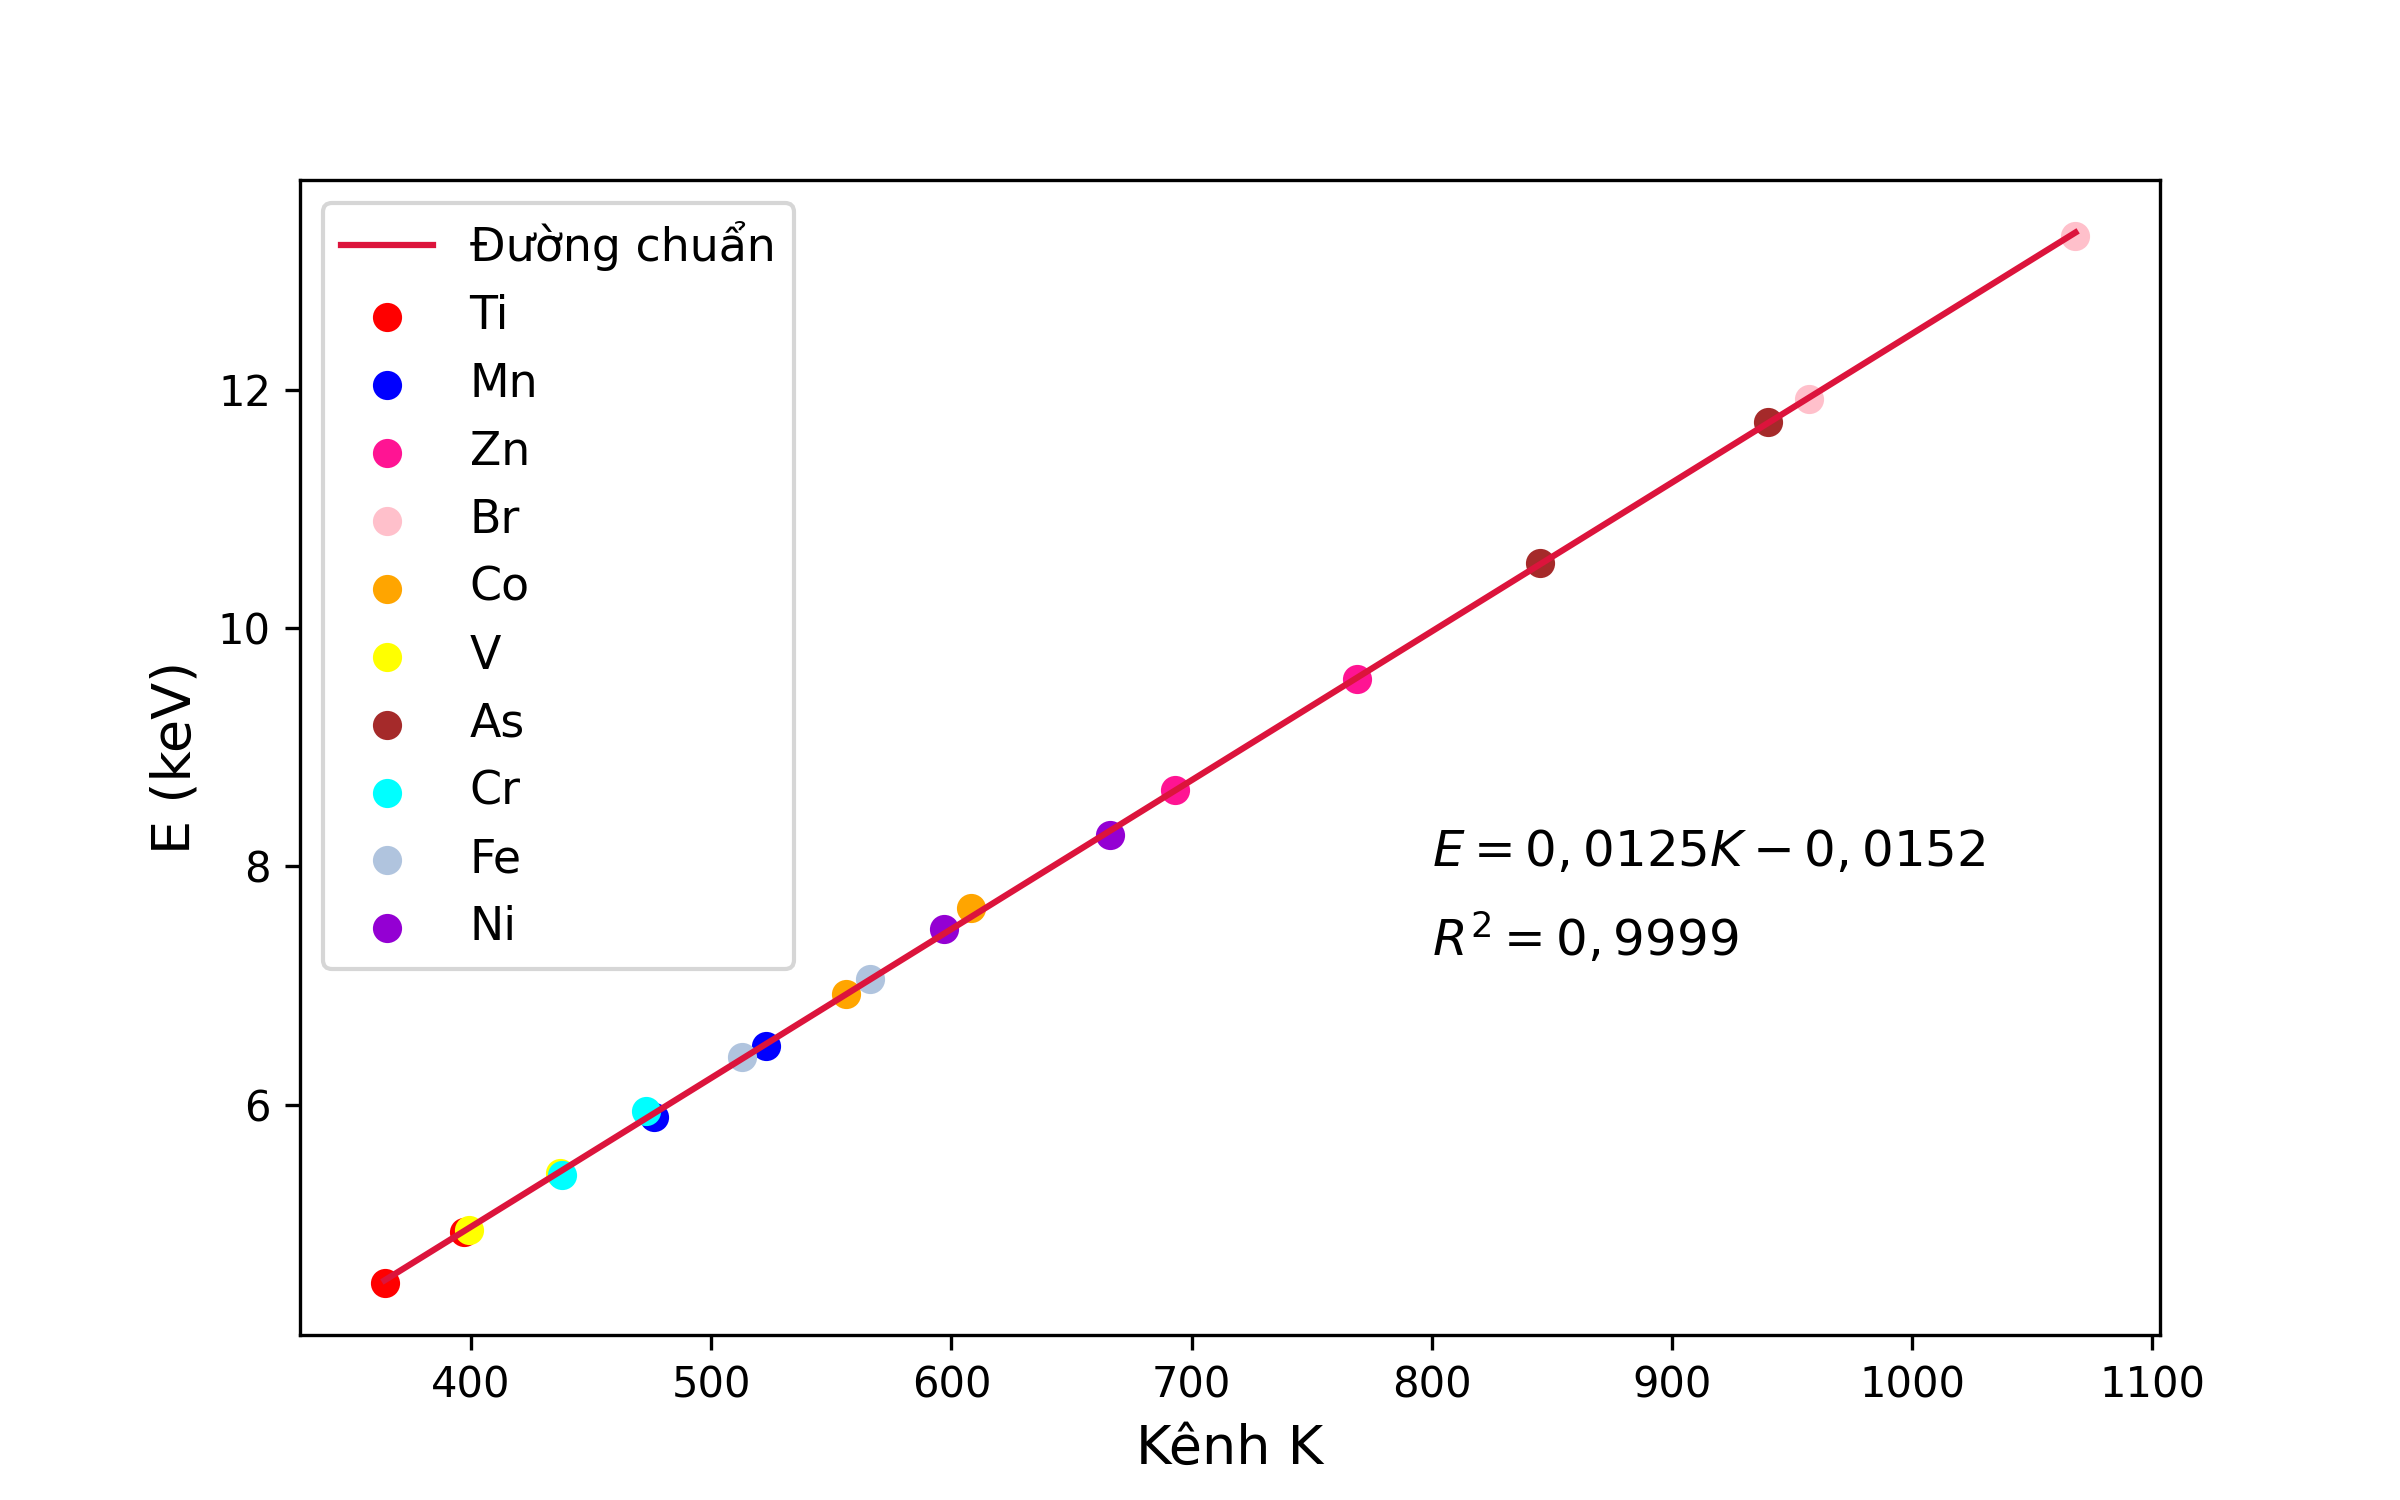
\includegraphics[width=\linewidth]{plot}
  \caption{Phương trình chuẩn năng lượng}
\end{figure}
\\ \par
\newpage
Từ đây ta có bảng số liệu nguồn X
% Please add the following required packages to your document preamble:
% \usepackage{multirow}

\begin{table}[h]
\centering
\begin{tabular}{|c|c|c|c|}
\hline
            & Kênh & Năng lượng (keV) & \multicolumn{1}{l|}{Tên nguồn X} \\ \hline
$K_{\alpha 1}$ & 644  & 8,02             & \multirow{2}{*}{Cu}              \\ \cline{1-3}
$K_{\beta }$  & 709  & 8,84             &                                  \\ \hline
$L_{\alpha 1}$    & 777  & 9,68             & \multirow{2}{*}{Ir}              \\ \cline{1-3}
$L_\beta $     & 845  & 10,53            &                                  \\ \hline
$K_{\alpha 1}$    & 957  & 11,93            & \multirow{2}{*}{Br}              \\ \cline{1-3}
$K_\beta $     & 1010 & 12,59            &                                  \\ \hline
\end{tabular}
\end{table}
\newpage
\clearpage\thispagestyle{empty}\addtocounter{page}{-1} 
\clearpage
\mbox{}
 % creates a blank space to fill the page
\newpage
\end{document}